\documentclass[11pt,a4paper]{article}
\usepackage[margin=2.1cm]{geometry}
\usepackage{amsmath,amssymb}
\usepackage{booktabs}
\usepackage{graphicx}
\usepackage{textcomp}
\usepackage[hidelinks]{hyperref}
\newcommand{\E}{\mathbb{E}}
\newcommand{\Prob}{\mathbb{P}}
\newcommand{\meur}{M\texteuro}
\newcommand{\code}[1]{\texttt{#1}}
\graphicspath{{../output/round1/figures/}}

\title{Lending Game -- Stage 1: the final pricing rule\\[2pt]
\large Pricing the pool we actually win -- Team ``Lender 2''}
\author{Internal note; supersedes the band section of the stage-1 strategy note}
\date{14 October 2026 (revised: income effect measured, 500-draw simulation)}

\begin{document}
\maketitle

\section{The rule, step by step}
We are one of three lenders bidding on the same 100,000 applicants. Each applicant takes the cheapest offer (with a
2\% preference for one lender), repays with interest or defaults and costs us the whole loan. Every lender sees the same
public variables and \emph{one private signal of its own}; the other two lenders' signals are information we do not have.
Our rule prices each applicant in five steps.

\paragraph{Step 1 -- estimate the probability of default.} A gradient-boosted tree model, trained on the 100,000 past
loans, gives $\hat p$ = the probability that the applicant defaults, from employment, marital status, income and our
signal $s_2$ (a signal of exactly 0 is treated as ``no signal''). It is well calibrated: among applicants with
$\hat p = 10\%$, 10\% default. Out-of-sample AUC 0.735.

\paragraph{Step 2 -- the plain break-even rate.} A loan at rate $r$ earns $10{,}000\,r$ if repaid and loses $10{,}000$ if
not, so it breaks even when $(1-\hat p)\,r = \hat p$, i.e. at $r = \hat p/(1-\hat p)$: 5.3\% for a 5\% PD, 11\% for 10\%,
25\% for 20\%. This is the rate a lender would charge if the applicants who accept were a random sample.

\paragraph{Step 3 -- the adjusted break-even: who actually accepts?} They are not a random sample. Each rival sees a
signal we do not; when that signal is bad the rival asks for more, and the applicant comes to us. So the applicants who
accept our offer are riskier than $\hat p$, and the more so the riskier the segment. We measured this on the past loans,
where all three signals are visible (Section~2): the default rate of the people \emph{we win} is $\tilde\pi(\hat p)$ --
12.7\% for applicants we rate at 10\%, 18\% at 15\%, 27\% at 20\%, 39\% at 25\%, above 50\% beyond 27\%. The
\emph{adjusted break-even} $\tilde\pi/(1-\tilde\pi)$ is the rate at which winning these applicants still breaks even:
13.7\% at $\hat p = 10\%$ instead of 11.1\%, 36\% at 20\% instead of 25\%, and no finite rate beyond 27\%. At a given PD
the curve also differs by income segment -- the pool we win is worse where a high PD is unusual for the segment; we
measured this (Section~2.1) and kept the single, pooled curve for the stage-1 file.

\paragraph{Step 4 -- the margin.} On safe applicants (up to a threshold $\tau$ of 8--12\% PD at low income, 25\% above
20k of income, Table~\ref{tab:params}) the rivals compete within a couple of points and the 2\% preference means we only
keep our own third of the market if we stay close to them: the margin is 3--4 points over the plain break-even, which is
about 2 points over the adjusted one. Above the threshold the rivals progressively stop competing (their own thresholds
lie between 8\% and 20\%), their prices disperse, and a larger margin captures more surplus without losing share: the
margin rises smoothly to $X = 5$ points over the adjusted break-even, the rise being centred one point above the threshold
and spread over about 8--14\% PD. $X = 5$ points was chosen by simulation (Section~3): a larger $X$ earns more when we are
the cheapest but is undercut more often by rivals pricing the same way.

\paragraph{Step 5 -- the cap.} No rate exceeds 0.989. In this game an applicant who receives at least one offer always
borrows, so a capped offer is a harmless ``lender of last resort'' quote: it is taken only if both rivals refuse the
applicant or quote above 0.989, and 0.989 beats a rival who caps at the obvious 0.99 or 1.00. It concerns 2\% of
applicants (2,027; PD above $\sim$27\%), for whom no finite competitive rate exists.

\paragraph{The formula.} With $s$ the income segment, $m(s)$ and $\tau(s)$ from Table~\ref{tab:params},
\begin{align}
r_{\text{safe}}(\hat p) &= \frac{\hat p}{1-\hat p} + m(s), \qquad
r_{\text{band}}(\hat p) = \min\!\Big(\frac{\tilde\pi(\hat p)}{1-\tilde\pi(\hat p)} + X,\; 0.989\Big), \qquad X = 0.05,\\[4pt]
r(\hat p) &= r_{\text{safe}} + w(\hat p)\,\big(r_{\text{band}} - r_{\text{safe}}\big), \qquad
w(\hat p) = \frac{1}{1+\exp\!\big(-(\hat p - \tau(s) - 0.01)/0.01\big)} .
\label{eq:rule}
\end{align}
$w$ is a logistic weight: 0.05 two points below the threshold, 0.27 at the threshold, 0.5 one point above it, 0.88 three
points above, 0.95 four points above. Rates are rounded to four decimals; every applicant receives an offer.

\begin{table}[h]\centering\small
\begin{tabular}{lcccccc}
\toprule
Income segment & 0 & 1--5k & 5--10k & 10--20k & 20--40k & 40k+\\
\midrule
margin $m(s)$ on the safe part & 4.0\% & 3.5\% & 3.5\% & 3.0\% & 3.0\% & 3.0\%\\
threshold $\tau(s)$ & 12\% & 12\% & 10\% & 8\% & 25\% & 25\%\\
share of the segment above the threshold (new file) & 92\% & 74\% & 69\% & 18\% & 0\% & 0\%\\
\bottomrule
\end{tabular}
\caption{Segment parameters, chosen by maximizing expected profit over competitor scenarios on the past loans. Thresholds
are low where the rivals' hidden information is large (standard deviation of $p^{\text{full}}-\hat p$: 7 points at zero
income, 0.3 points above 40k).}
\label{tab:params}
\end{table}

\begin{table}[h]\centering\small
\resizebox{\textwidth}{!}{%
\begin{tabular}{crrrrl}
\toprule
PD $\hat p$ & plain break-even & adjusted break-even & margin over adjusted & \textbf{rate offered} & what happens\\
\midrule
6\%  & 6.4\%  & 7.5\%  & 2.4 pts & \textbf{9.9\%}  & competitive pricing, we keep our fans\\
8\%  & 8.7\%  & 10.6\% & 1.8 & \textbf{12.4\%} & idem\\
10\% & 11.1\% & 13.7\% & 2.0 & \textbf{15.7\%} & threshold: the margin starts to rise\\
12\% & 13.6\% & 16.4\% & 3.9 & \textbf{20.3\%} & rivals begin to drop out\\
14\% & 16.3\% & 21.2\% & 4.7 & \textbf{25.9\%} & \\
16\% & 19.0\% & 27.1\% & 4.9 & \textbf{32.1\%} & full margin: adjusted break-even + 5\\
20\% & 25.0\% & 36.1\% & 5.0 & \textbf{41.1\%} & \\
25\% & 33.3\% & 64.7\% & 5.0 & \textbf{69.7\%} & the selected pool defaults 39\%\\
30\% & 42.9\% & none below 100\% & -- & \textbf{98.9\%} & cap: taken only if both rivals refuse\\
\bottomrule
\end{tabular}}
\caption{The rule at a glance, for an applicant with income 5--10k (threshold 10\%, margin 3.5\%). Example: income
7,000~\texteuro{}, PD 12\%: plain break-even $0.12/0.88 = 13.6\%$; the applicants we would win at that PD default 14.1\%, so the
adjusted break-even is $0.141/0.859 = 16.4\%$; the margin at 12\% PD is 3.9 points; offer 20.3\%.}
\label{tab:glance}
\end{table}

\section{Where $\tilde\pi$ comes from: the break-even given that we win}
\paragraph{The measurement.} For every past loan $i$ we compute the three lenders' out-of-sample estimates
$\hat p_{k,i} = \E[D \mid X, s_k]$, $k=1,2,3$ (each with its own signal), and a \emph{full-information} estimate
$p^{\text{full}}_i = \E[D \mid X, s_1, s_2, s_3]$ from a model trained on all three signals (out-of-sample as well).
$p^{\text{full}}$ is a diagnostic estimate, not the truth: it is the best available stand-in for the default probability
that the three signals together carry; its realized counterpart $D_i$ is used to check it. We let every lender quote
$\hat p_{k,i}/(1-\hat p_{k,i}) + m(s_i)$ -- the same rule, each on its own information -- and apply the choice rule of the
game for each applicant type $t\in\{1,2,3\}$ (one third each; the preferred lender's rate counts 0.02 lower):
\begin{equation}
\omega_i \;=\; \frac{1}{3}\sum_{t=1}^{3} \mathbf 1\Big\{\, r_{2,i} - 0.02\cdot\mathbf 1[t=2] \;<\; \min_{k\neq 2}\big(r_{k,i} - 0.02\cdot\mathbf 1[t=k]\big) \Big\}
\end{equation}
is the probability that applicant $i$ takes our offer (``share we win'' in Table~\ref{tab:curse} is its average). For
each PD bin $B$ (one point wide),
\begin{equation}
\tilde\pi(B) = \frac{\sum_{i\in B}\omega_i\, p^{\text{full}}_i}{\sum_{i\in B}\omega_i},
\qquad
\tilde\pi^{\text{real}}(B) = \frac{\sum_{i\in B}\omega_i D_i}{\sum_{i\in B}\omega_i},
\qquad
\tilde\pi^{95}(B) = \tilde\pi^{\text{real}} + 1.645\sqrt{\frac{\tilde\pi^{\text{real}}(1-\tilde\pi^{\text{real}})}{\sum_{i\in B}\omega_i}} .
\end{equation}
$\tilde\pi$ is the default rate of the applicants we win; the expected version (with $p^{\text{full}}$, smoothed with a
three-bin rolling mean) is used in the rule, the realized version and its 95\% upper bound check it (Table~\ref{tab:curse},
Figure~\ref{fig:A}A).

\begin{table}[h]\centering\small
\resizebox{\textwidth}{!}{%
\begin{tabular}{crccccc}
\toprule
Our PD $\hat p$ & Share we win & $\tilde\pi$ (expected) & $\tilde\pi^{95}$ (realized, upper) & Penalty $\tilde\pi-\hat p$ & Plain break-even & Adjusted break-even\\
\midrule
5\%  & 44\% & 5.1\%  & 5.5\%  & +0.6 pt & 4.7\%  & 5.3\%\\
8.5\% & 39\% & 10.2\% & 11.3\% & +1.7 & 9.2\% & 11.3\%\\
10.5\% & 38\% & 12.7\% & 14.2\% & +2.1 & 11.7\% & 14.5\%\\
12.5\% & 44\% & 14.4\% & 15.8\% & +1.9 & 14.3\% & 16.9\%\\
14.5\% & 29\% & 18.2\% & 19.9\% & +3.7 & 16.9\% & 22.2\%\\
16.5\% & 17\% & 22.9\% & 26.7\% & +6.4 & 19.7\% & 29.6\%\\
18.5\% & 18\% & 24.1\% & 27.9\% & +5.6 & 22.7\% & 31.7\%\\
20.5\% & 11\% & 26.9\% & 30.1\% & +6.5 & 25.7\% & 36.8\%\\
22.5\% & 18\% & 29.0\% & 37.0\% & +6.5 & 29.1\% & 40.8\%\\
24.5\% & 13\% & 35.5\% & 39.7\% & +11.0 & 32.5\% & 55.0\%\\
26.5\% & 4\%  & 46.8\% & 58.2\% & +20.2 & 36.2\% & 88.1\%\\
$\ge 28\%$ & $\le 1\%$ & $> 50\%$ & -- & $> 20$ & $\ge 40\%$ & none below the cap\\
\bottomrule
\end{tabular}}
\caption{The winner's curse per PD level, all income segments pooled, measured on the past loans when every lender prices
on its own model.}
\label{tab:curse}
\end{table}

Three remarks. (i) If every lender applied the same strictly increasing transformation to its own PD and there were no
preference, the same applicants would be won whatever the common margin, and $\tilde\pi$ would not depend on the rivals'
rule at all. With the 2\% preference this holds only approximately: two points of rate correspond to different PD gaps
under a steep and under a flat rule. We therefore recomputed $\tilde\pi$ under five other common rules (the submitted rule
itself applied by everyone, the lecture formula $\hat p + 3\%$, twice the break-even, break-even $+10\%$, and no
preference): the curve moves by at most 1.7 points of default over 5--25\% PD, 0.3 on average -- covered by the
five-point margin. What $\tilde\pi$ does depend on is the rivals' models being about as informative as ours. (ii) The
curse is small where our model can compete (below 10\% PD the penalty is at most 2 points) and explodes above 25\%:
beyond $\sim$27\% the applicants we would win in competition default more than half the time and no finite rate breaks
even. (iii) The 95\% upper bound stays within 1--4 points of the expected curve up to 25\% PD, so the five-point margin
also covers the estimation uncertainty there.

\subsection{Does the curve depend on income? Measured, not adopted for stage 1}
At the same PD, the pool we win is not the same in every segment (Table~\ref{tab:seg}, Figure~\ref{fig:C}A). Among
applicants we rate at 12--13\%, those we win default 13.5\% at zero income (1,196 expected wins in the bin), 16.1\% at
5--10k (722) and 26\% at 10--20k (12, a thin bin); at 16--17\%, 19.9\% versus 26.0\%. The reason is the intensity of the
selection, and it shows in how often we win. A PD of 12\% is below the typical risk of a zero-income applicant (the
segment averages 20\%): the rivals, who see the income but not our signal, usually estimate him higher than we do (17\%
on average), so we win him 69\% of the time, including every case where their signals are merely neutral -- little
selection, small curse. The same 12\% is far above the typical risk of a 10--20k applicant (6\%): the rivals usually
estimate him around 9\%, undercut us, and we win only 4\% of the time, precisely when both of their signals are bad as
well -- those few applicants default 26\%. The realized defaults show the same pattern (13.5\%, 16.6\% and 24\%).

To quantify it we fitted one curve per income segment: on the logit scale, the pooled curve shifted by a
segment-specific amount that varies linearly with $\operatorname{logit}\hat p$,
\begin{equation}
\operatorname{logit}\tilde\pi_s(\hat p) = \operatorname{logit}\tilde\pi(\hat p) + \alpha_s + \beta_s\big(\operatorname{logit}\hat p - \operatorname{logit}0.12\big),
\end{equation}
with $(\alpha_s,\beta_s)$ fitted by weighted least squares on the probability scale (weights $\omega_i$, target
$p^{\text{full}}_i$) over the PD range from three points below the segment's threshold up to the last one-point bin with
at least 20 expected wins (9--28\% at zero income, 9--19\% at 1--5k, 7--20\% at 5--10k, 5--12\% at 10--20k); beyond
that range the shift is held constant rather than extrapolated; the 20--40k and 40k+ segments have no past loans won
above their 25\% threshold and keep the pooled curve. Fitted shifts: $\alpha = -0.12, -0.08, +0.09, +0.33$ and
$\beta = +0.07, +0.34, +0.34, +0.43$ for zero income, 1--5k, 5--10k, 10--20k.

\begin{table}[h]\centering\small
\resizebox{\textwidth}{!}{%
\begin{tabular}{lccccc|ccccc}
\toprule
 & \multicolumn{5}{c|}{$\tilde\pi_s$: default rate of the applicants we win} & \multicolumn{5}{c}{adjusted break-even $\tilde\pi_s/(1-\tilde\pi_s)$}\\
Our PD $\hat p$ & 0 & 1--5k & 5--10k & 10--20k & pooled & 0 & 1--5k & 5--10k & 10--20k & pooled\\
\midrule
12\% & 12.7\% & 13.1\% & 15.3\% & 18.6\% & 14.1\% & 14.6\% & 15.1\% & 18.0\% & 22.8\% & 16.4\%\\
16\% & 19.7\% & 21.9\% & 24.9\% & 27.3\% & 21.3\% & 24.6\% & 28.0\% & 33.2\% & 37.6\% & 27.1\%\\
20\% & 25.0\% & 28.6\% & 32.7\% & 33.4\% & 26.5\% & 33.4\% & 40.1\% & 48.6\% & 50.1\% & 36.1\%\\
25\% & 37.9\% & 41.8\% & 46.5\% & 47.3\% & 39.3\% & 61.1\% & 71.7\% & 87.0\% & 89.7\% & 64.7\%\\
PD at which the band would reach the cap & & & & & & 28.0\% & 26.5\% & 25.5\% & 25.5\% & 27.5\%\\
\bottomrule
\end{tabular}}
\caption{The selected default rate and the adjusted break-even by income segment, from the fitted curves
(\code{output/round1/curse\_floor\_by\_segment.csv}); ``pooled'' is the curve used in the submitted file.}
\label{tab:seg}
\end{table}

\paragraph{Is the segment effect real?} Two-fold check: the past loans are split at random into halves, the pooled curve
and the shifts are re-estimated on one half and compared with the raw bin values of the other half in the band region. The
pooled curve is biased by $+1.4$ to $+1.5$ points of default at zero income (too high), $-0.8$ to $-1.3$ at 5--10k and
$-1.2$ to $-1.3$ at 10--20k (too low); the segment curves fitted on the other half are unbiased within 0.5 point in every
segment and both folds, and their mean absolute error falls from 1.2 to 0.5 point. The shifts themselves are stable across
the two halves. So, relative to the pool it actually wins, the pooled rule over-prices the zero-income band by 1--3 points
and under-prices the 5--10k band above $\sim$15\% PD and the 10--20k band above $\sim$11\% PD, where the pooled rate falls
below the segment's break-even. An income-conditioned file would price the band 1--3 points lower at zero income, 0.5
(10--12\% PD) to 16 points (22--25\% PD) higher at 5--10k and 1 to 13 points higher at 10--20k.

\paragraph{Why it is not in the stage-1 file.} Evaluated on the same simulated markets as the submitted rule
(Section~3.1), the income-conditioned curve adds $+0.46 \pm 0.02$~\meur{} prior-weighted at $X = 0.05$ (it earns 0.25 less
against rivals who price like us on the pooled curve, because they take some thinly profitable 5--10k loans from it, and
0.1--1.9 more in every other profile) and lowers the probability of finishing last from 1.6\% to 0.7\% at an unchanged
78\% probability of finishing first. The team nevertheless kept the single pooled curve for stage 1: the gain is 3\% of
the expected profit and comes from the profiles we weight less; the largest shifts (10--20k above 12\% PD, 2,300 offers)
are extrapolated from thin bins; and one curve is easier to explain and to revise once the rivals' actual prices are
observed. The income-conditioned curve is the first candidate for stage 2; its files are kept in
\code{output/round1/alternatives/}.

\begin{figure}[h]\centering
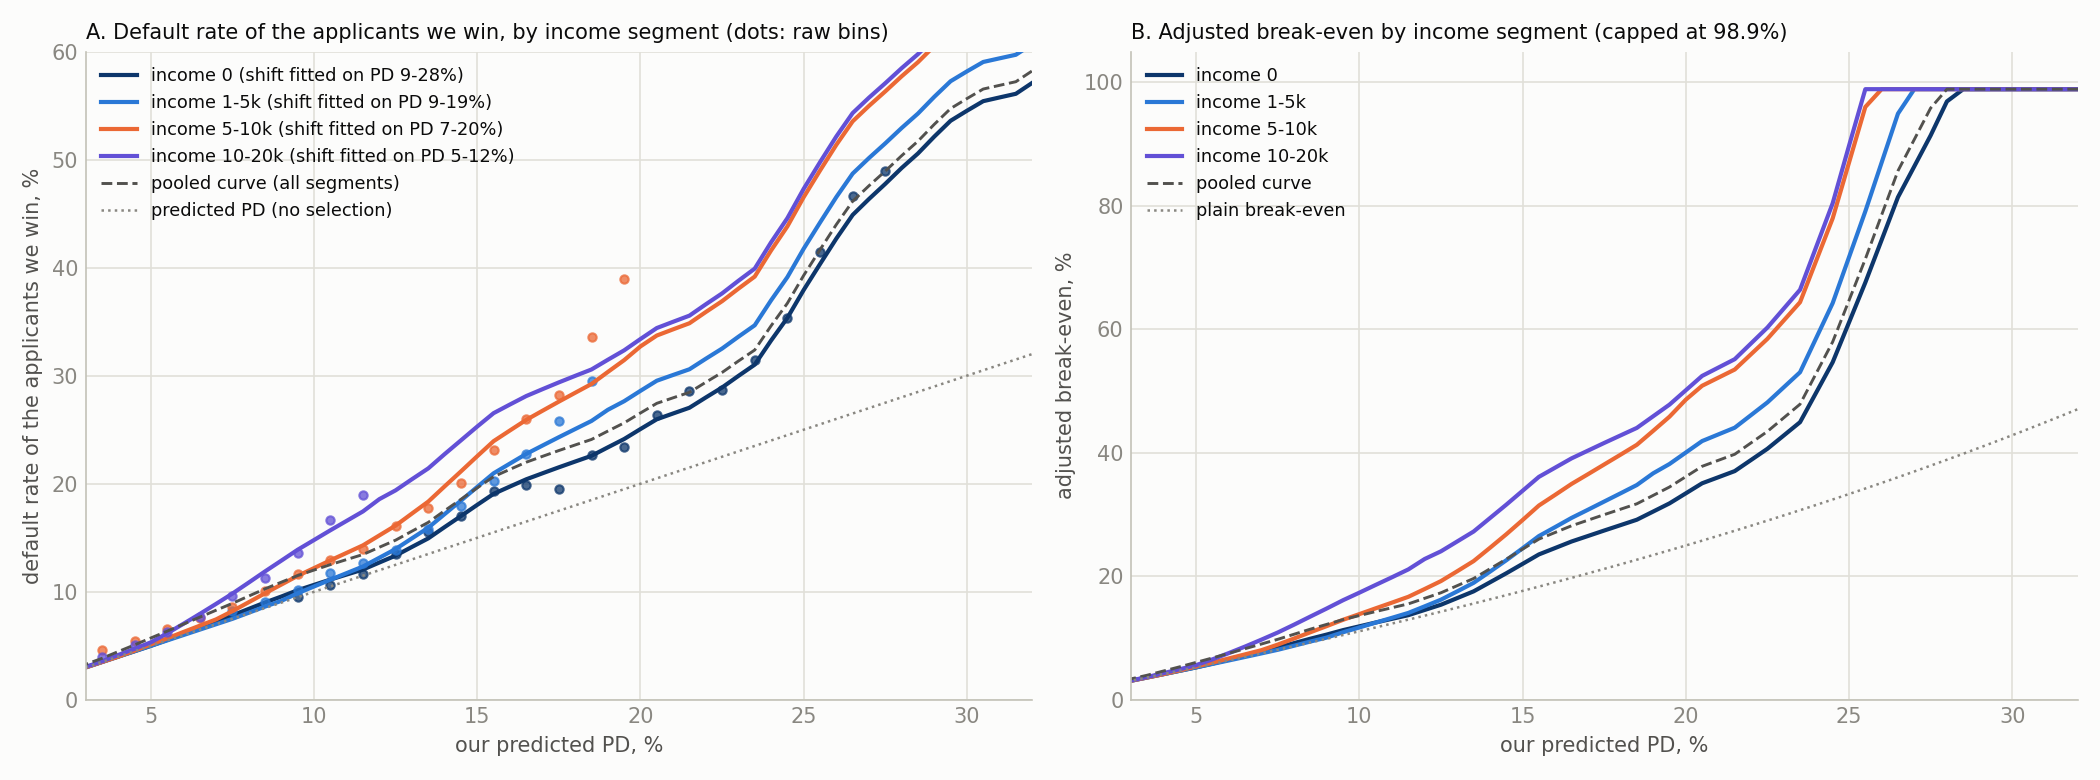
\includegraphics[width=\textwidth]{figC_curse_by_segment.png}
\caption{A: the default rate of the applicants we win, by income segment -- lines: the fitted curves, dots: raw one-point
bins with at least 20 expected wins, dashed: the pooled curve used in the file. B: the resulting adjusted break-even by
segment, capped at 98.9\%.}
\label{fig:C}
\end{figure}

\begin{figure}[h]\centering
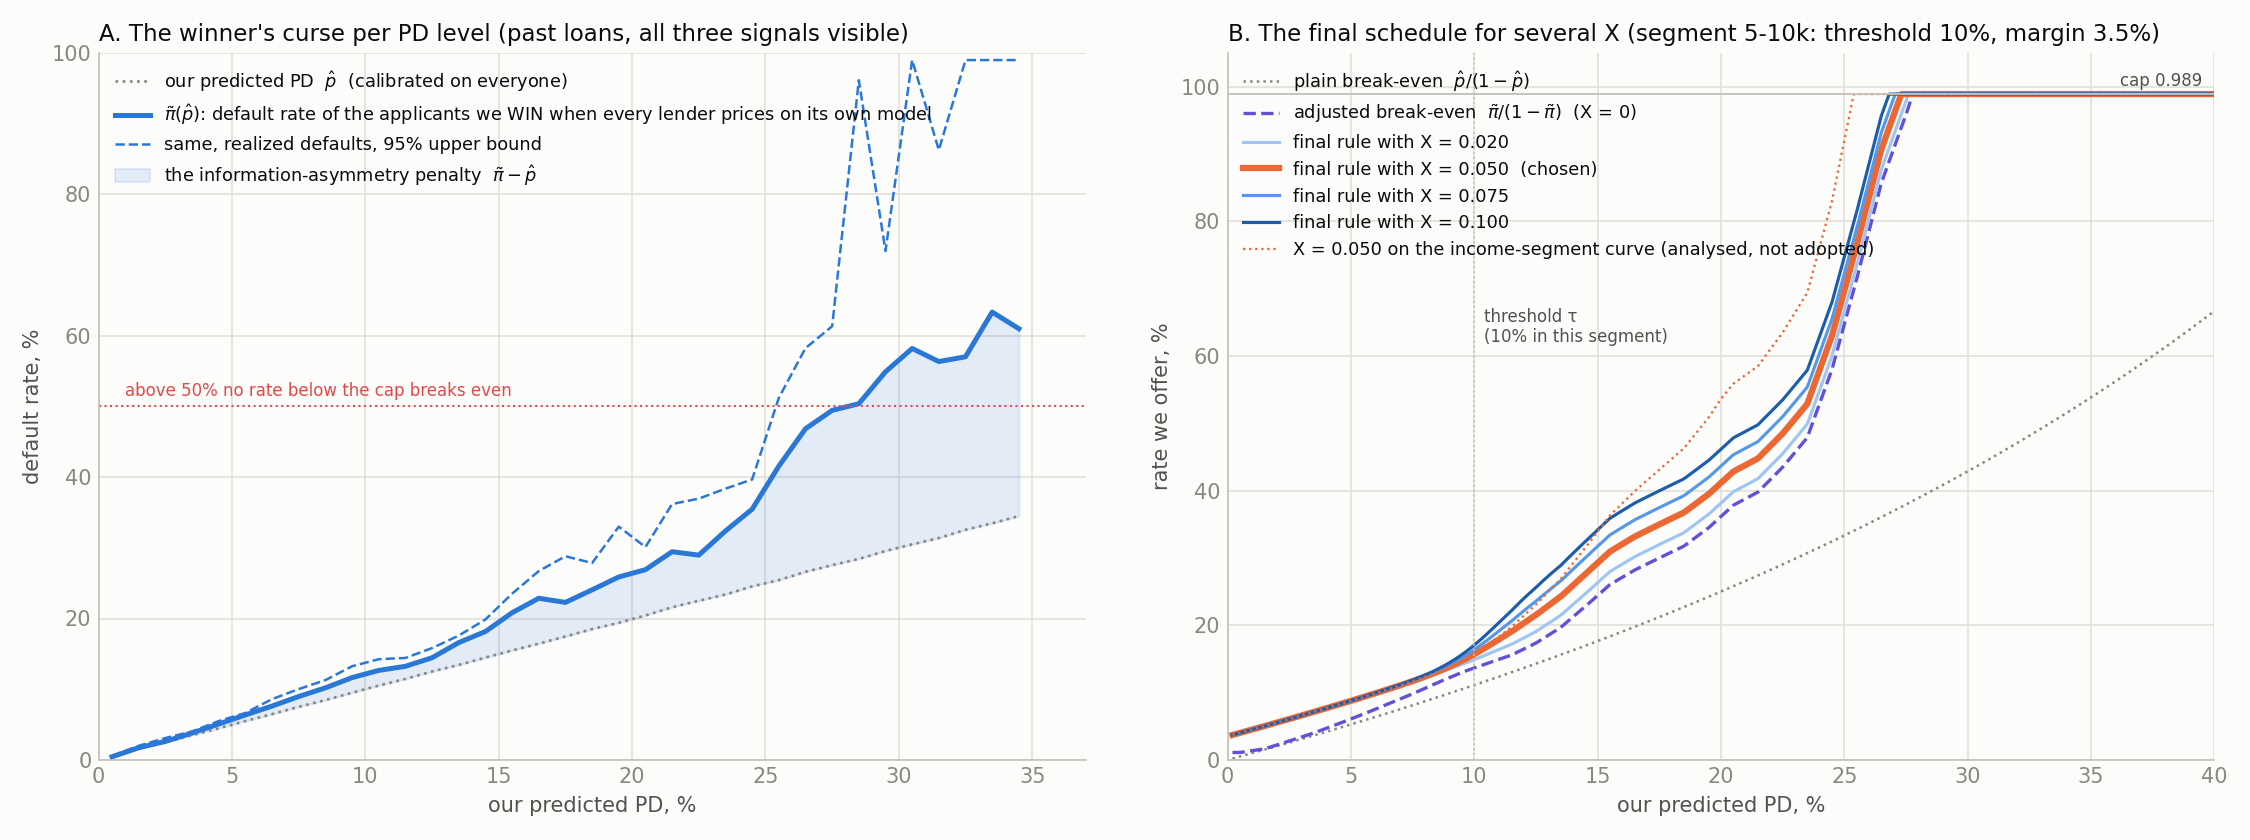
\includegraphics[width=\textwidth]{figA_curse_and_rule.png}
\caption{A: our predicted PD versus the default rate of the applicants we win, all segments pooled (expected, and realized
95\% upper bound); the shaded area is the price of the information asymmetry. B: the final schedule in the 5--10k segment
(threshold 10\%, margin 3.5\%) for several margins $X$; $X = 0.05$ is the submitted rule; the dotted line is the same $X$
on the income-segment curve of Section~2.1 (analysed, not adopted).}
\label{fig:A}
\end{figure}

\section{Choosing the margin $X$ and its transition}
\subsection{The level of $X$: a Monte Carlo over rival strategies}
At $X = 0$ we would break even on the band even if we won all of it; the margin is what we earn there. But every point of
margin is a point by which a rival pricing the same way can undercut us, and with the 2\% preference whoever is lowest
within two points takes the whole band. So $X$ is a bet on the rivals' margins. Each rival is drawn at random from a
profile of plausible behaviours and priced on its own PD estimate; the market is evaluated exactly (three applicant types
with weight $1/3$, ties split evenly -- an adverse-tie variant gives identical results, since the schedules create no
exact ties), rates rounded as in the file, profits computed with $p^{\text{full}}$. Profiles and weights (our belief that
the rivals are curse-aware and do not use a lender-of-last-resort rate): \emph{like us, no net} -- rivals pricing the band
at their own adjusted break-even plus a margin drawn between 3 and 25 points (40\%); \emph{smart} -- curse-aware rivals
using a net, a ramp, a large margin, a data-driven schedule, refusal or a compromise (20\%); \emph{clones} of our method
with other parameters (10\%); \emph{best-responders} who undercut our schedule (10\%); a broad \emph{mixed} profile
including naive behaviours (10\%); pure \emph{netters} (5\%); \emph{model-followers} pricing model + 2--6\% for everyone
(5\%). A first pass used 120 rival pairs per profile, too few to resolve probabilities of 1--3\%; the final pass uses 500
per profile (3,500 markets), with standard errors, and evaluates the income-segment curve of Section~2.1 on the same draws.

\begin{table}[h]\centering\small
\resizebox{\textwidth}{!}{%
\begin{tabular}{lccc|ccc}
\toprule
 & \multicolumn{3}{c|}{Prior-weighted over the seven profiles} & \multicolumn{3}{c}{``Like us, no net'' rivals only}\\
Band schedule & mean profit (s.e.) & P(first) & P(last) (s.e.) & mean profit & P(first) & P(last)\\
\midrule
pooled curve, $X = 0.03$ & 14.2 (0.1) & 84\% & 1.0\% (0.3) & 11.6 & 72\% & 2.6\%\\
\textbf{pooled curve, $X = 0.05$ (submitted)} & \textbf{15.5 (0.1)} & \textbf{78\%} & \textbf{1.6\% (0.3)} & \textbf{12.4} & \textbf{62\%} & \textbf{3.6\%}\\
pooled curve, $X = 0.075$ & 16.8 (0.1) & 70\% & 3.4\% (0.5) & 12.9 & 47\% & 7.6\%\\
\midrule
income-segment curve (Section~2.1), $X = 0.02$ & 14.2 (0.1) & 84\% & 0.3\% (0.2) & 11.2 & 69\% & 0.8\%\\
income-segment curve, $X = 0.03$ & 14.8 (0.1) & 83\% & 0.3\% (0.2) & 11.5 & 67\% & 0.8\%\\
income-segment curve, $X = 0.05$ & 15.9 (0.1) & 78\% & 0.7\% (0.2) & 12.1 & 58\% & 1.8\%\\
income-segment curve, $X = 0.075$ & 17.1 (0.2) & 70\% & 2.7\% (0.4) & 12.6 & 44\% & 6.2\%\\
income-segment curve, $X = 0.10$ & 18.1 (0.2) & 64\% & 5.4\% (0.6) & 12.8 & 34\% & 12.6\%\\
\bottomrule
\end{tabular}}
\caption{Expected profit and rank among the three lenders as a function of the margin $X$, for the pooled curve (submitted)
and the income-segment curve of Section~2.1 (500 random rival pairs per profile, the same draws for every schedule).
Profit rises with $X$; the probability of finishing first falls with it.}
\label{tab:X}
\end{table}

\paragraph{The criterion.} Stage-1 performance is graded on the level of profit \emph{and} on the ranking, so we declared
the rule before the final runs: maximize the prior-weighted expected profit subject to a probability of finishing last of
at most 3\%. This is a constrained choice: the unconstrained maximum of the mean lies at a larger $X$ (and, in the first
pass, at the hand-made ramp 0.45--0.65, 22~\meur{} on average but last in 41\% of the draws because of jackpots against
netters and heavy losses against rivals who price like us). With 500 draws the limit binds between 0.05 and 0.075: the
probability of finishing last is 1.6\% (standard error 0.3) at $X = 0.05$ and 3.4\% (0.5) at $X = 0.075$, so the
criterion selects $X = 0.05$, as in the first pass; its one-sided 95\% bound, 2.1\%, is inside the limit. In expected
rank over the prior, $X = 0.05$ gives 1.24 and $X = 0.075$ 1.33, for a gain of 1.3~\meur{} (8\%) in expected profit. On
the income-segment curve the limit would be met at $X = 0.075$ at the point estimate (2.7\%) but not with its margin
(3.4\%). Figure~\ref{fig:B} shows the dial.

\begin{figure}[h]\centering
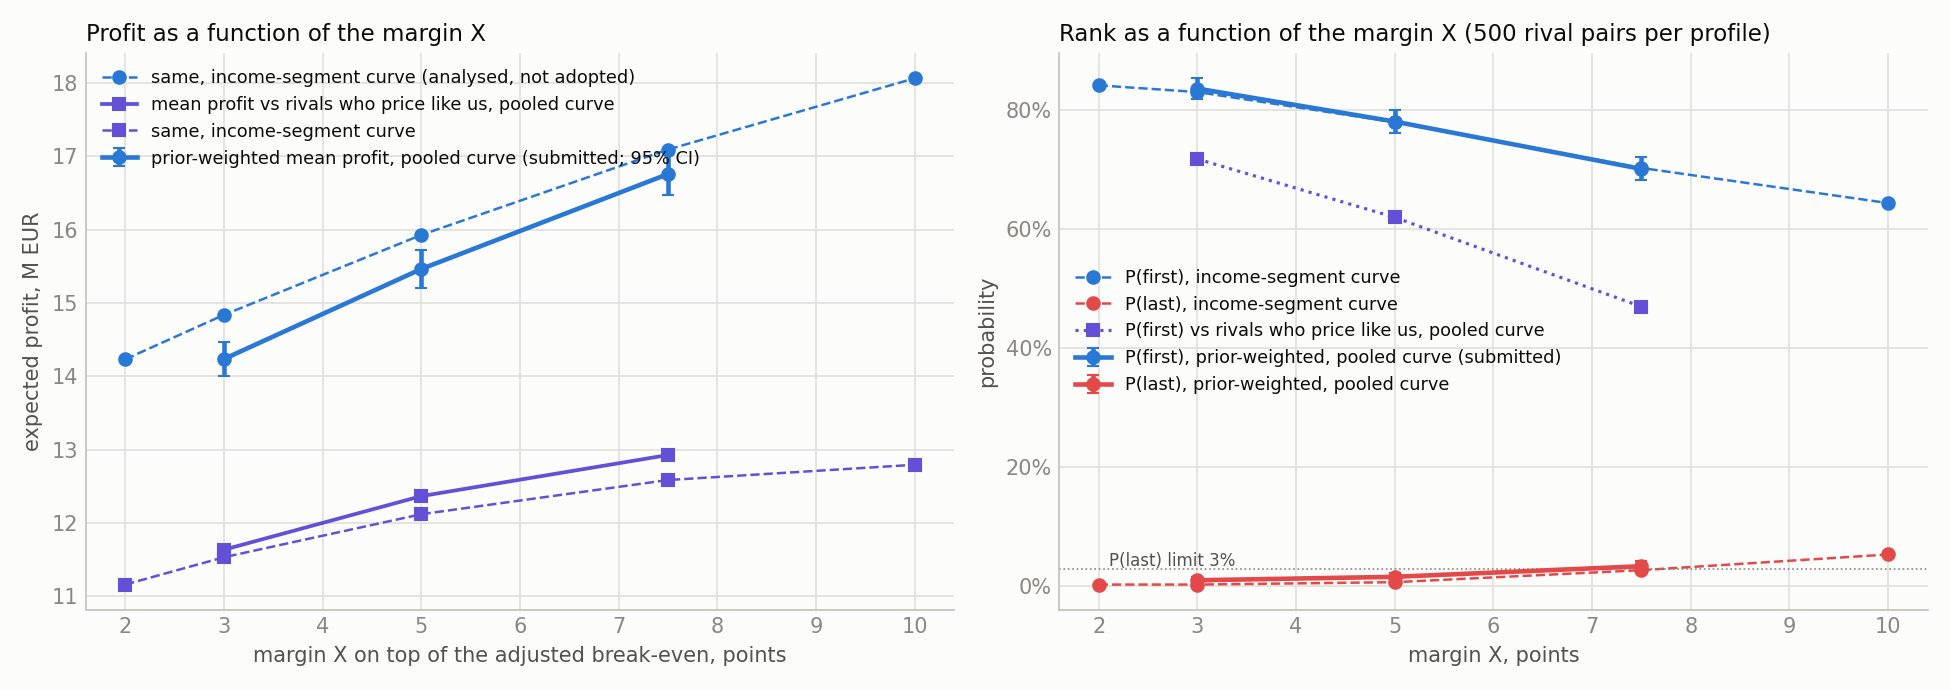
\includegraphics[width=0.95\textwidth]{fig13b_final_margin_v2.png}
\caption{Expected profit (left) and rank (right) as a function of the margin $X$ on top of the adjusted break-even, with
95\% confidence intervals from the 500 draws per profile; solid: pooled curve (submitted), dashed: income-segment curve of
Section~2.1.}
\label{fig:B}
\end{figure}

\subsection{The transition: where the margin rises}
A first version switched from the safe-part margin to the band margin in one point of PD at the threshold, which produced a
jump of five points in the rate between 10\% and 11\% PD (14.8\% to 19.7\% in the 5--10k segment) although the default rate
of the people we win moves by one point there -- an artefact of gluing two formulas, with no economic event behind it. We
therefore let the margin rise smoothly, and chose the width by the same Monte Carlo:

\begin{table}[h]\centering\small
\resizebox{\textwidth}{!}{%
\begin{tabular}{lcccc}
\toprule
Transition of the margin & rate at 10 / 11 / 12 / 14\% PD & prior-weighted mean & P(first) & P(last)\\
\midrule
one-point step at the threshold & 14.8 / 19.7 / 21.4 / 26.2 & 16.3~\meur{} & 82\% & 1\%\\
\textbf{logistic, centre $\tau$+1 pt, scale 1 pt (submitted)} & \textbf{15.7 / 17.9 / 20.3 / 25.9} & \textbf{15.8} & \textbf{82\%} & \textbf{1\%}\\
logistic, centre $\tau$+2, scale 1.5 & 15.4 / 17.2 / 19.3 / 24.9 & 15.2 & 83\% & 2\%\\
logistic, centre $\tau$+3, scale 2.5 & 15.6 / 17.1 / 18.9 / 23.6 & 14.4 & 83\% & 2\%\\
\bottomrule
\end{tabular}}
\caption{Smoothing the margin transition (100 random rival pairs per profile, segment 5--10k for the rates).}
\end{table}

The submitted transition (spread over roughly 8--14\% PD) costs 0.5~\meur{} of expected profit -- inside the simulation's
noise -- and nothing in rank; wider transitions give margin away to applicants most rivals have already stopped competing
for. Economically the width matches where rivals disengage: their thresholds, in every profile we consider, lie between
8\% and 20\% PD and concentrate around 10--12\%.

\subsection{The cap: are the capped offers profitable?}
Above $\sim$27\% PD the adjusted break-even plus five points exceeds 98.9\%, so the rule caps the rate at 0.989 for about
2\% of applicants (2,027 in the submitted file; 1,946 of the past loans on which the simulations below run). Does that
mean we lose money on them? No -- the two statements concern two different pools. The adjusted break-even is the
break-even of the applicants we would win \emph{in competition}, i.e.\ because our estimate is the lowest of the three;
above 27\% PD that pool defaults more than half the time, which is exactly why the rule stops competing there. At 0.989
we are the cheapest only when \emph{both rivals refuse the applicant or quote above 0.989}: a pool selected by the rivals'
refusal rules, not by our estimate being the lowest. Table~\ref{tab:cap} measures it: where we win any capped loans their
expected default is 33--46\%, below the 50\% at which a 98.9\% loan breaks even; the one profile with a worse pool
(model-followers, 59\%) yields two loans. Prior-weighted, keeping the cap earns $+0.10$~\meur{}, refusing those
applicants 0, capping only up to 30\% PD $+0.06$~\meur{}. The cap is kept: a small option, not negative in any profile
we simulated except model-followers ($-0.003$~\meur{}).

\begin{table}[h]\centering\small
\begin{tabular}{lccc}
\toprule
Rival profile & expected loans won at the cap (of 1,946 offers) & their expected default & profit on them\\
\midrule
like us, no net & 122 & 46\% & $+0.10$~\meur{}\\
smart & 70 & 33\% & $+0.23$\\
mixed & 71 & 40\% & $+0.14$\\
netters & 26 & 33\% & $+0.09$\\
clones & 3 & 39\% & $+0.01$\\
best-responders & 0 & -- & 0\\
model-followers & 2 & 59\% & $-0.003$\\
\bottomrule
\end{tabular}
\caption{The capped offers by rival profile (exact types, fair ties, 60 rival pairs per profile).}
\label{tab:cap}
\end{table}

\section{The submitted file}
\code{output/round1/rates\_round1.csv}, built from the model refitted on all past loans (full-precision PDs) by
\begin{center}\code{python make\_submission.py --adjusted-x 0.05 --cap 0.989 --phase-delta 0.01 --phase-width 0.01}\end{center}
100,000 rows, columns \code{id} and \code{rate}, ids 1 to 100,000 in order and unique, no missing value, all rates in
$[0.0304, 0.989]$; the SHA-256 checksum (\code{5aba4d61...}) and the exact parameters are stored in
\code{rates\_round1\_params.json}. The income-conditioned files of Section~2.1 ($X = 0.05$ and $0.075$, built with the
option \code{--floor-by-segment}) are kept in \code{output/round1/alternatives/} and were not submitted.

\begin{table}[h]\centering\small
\resizebox{\textwidth}{!}{%
\begin{tabular}{lrrrrrrrrrr}
\toprule
rate & $\le$5\% & 5--10\% & 10--15\% & 15--20\% & 20--30\% & 30--40\% & 40--50\% & 50--60\% & 60--80\% & 80--98.9\%\\
\midrule
offers & 13,474 & 25,593 & 13,596 & 12,482 & 12,854 & 10,219 & 3,576 & 3,559 & 1,515 & 3,132\\
\bottomrule
\end{tabular}}
\caption{Composition of the file: 54,418 applicants below their segment's threshold (rates 3.0\% to 18.6\%) and 45,582
above it, priced on the adjusted break-even (12.8\% to 98.9\%), of which 2,027 at the cap.}
\end{table}

\section{What we expect, and what could go wrong}
Across the rival profiles the expected profit of this rule is 7--25~\meur{} (prior-weighted 15.5~\meur{}, 5th
percentile 7.9), finishing first in 78\% of the simulated markets and last in 1.6\%; against rivals who price like us,
12.4~\meur{}, first 62\%, last 3.6\%. The assumptions that matter most are (i) that the rivals' models are about as
informative as ours -- if theirs are worse, the curse is smaller and we are slightly over-pricing the band; if better, the
five-point margin is our cushion; (ii) that $p^{\text{full}}$, a model estimate, is a fair stand-in for the risk the three
signals carry -- the realized defaults agree with it within 0.5~\meur{} in aggregate and within the 95\% bounds of
Table~\ref{tab:curse}; (iii) the ``like us'' profile, which carries 40\% of our prior, is our own construct, and its
margins (uniform on 3--25 points) drive the choice of $X$ directly; (iv) the pooled curve under-states the cost of the
loans we win above $\sim$15\% PD at 5--10k and $\sim$11\% PD at 10--20k (Section~2.1): the five-point margin absorbs part
of it, and the simulation puts the cost of ignoring the income effect at about 0.5~\meur{}; (v) the rules as written: an
applicant with at least one offer always borrows, which is what makes the capped offers harmless. After stage 1 we will
read the rivals' actual band prices from the results and re-price each PD category at their observed level minus a few
points where that stays above the adjusted break-even -- by income segment if the stage-1 results support it -- which is
the only part of the rule that depends on a belief rather than on a measurement.
\end{document}
